%%%%%%%%%%%%%%%%%%%%%%%%%%%%%%%%%%%%%%%%%%%%%%%%%%%%%%%%%%%%%%%%%%%%%%
% Problem statement
\begin{statement}[
  problempoints=100,
  timelimit=1 sekunda,
  memorylimit=1024 MiB,
]{Ministarstvo}

Pero se nakon uspješne karijere u stranci koju nećemo imenovati, zaposlio u Ministarstvu turizma. Pero nadgleda mrežu od $N$ gradova, označenih brojevima od $1$ do $N$, gdje između svaka dva grada postoji točno jedna jednosmjerna cesta. Kako bi povećao prihode, odlučio je uvesti dozvole za prometovanje. Pero bi najradije uveo posebnu dozvolu za svaku cestu, no to bi alarmiralo njegove nadređene. Stoga, uvest će $K$ različitih dozvola, označenih od $1$ do $K$, te će za prolazak svakom cestom biti potrebno posjedovanje točno određene dozvole. 

Kako bi ipak osigurao pozamašne prihode, Pero će se zadovoljiti sa sljedećim svojstvom.

\begin{itemize}
\item Za svaki grad $v$ postoji neki grad $u$, tako da iz grada $v$ nije moguće doći do grada $u$ posjedovanjem samo jedne dozvole.
\end{itemize} 

Pero vas moli da mu pomognete, te da odredite najmanji $K$ takav da postoji pridruživanje dozvola s traženim svojstvom te neko takvo pridruživanje! Ako ne postoji takvo pridruživanje, ispišite \texttt{-1}. 

%%%%%%%%%%%%%%%%%%%%%%%%%%%%%%%%%%%%%%%%%%%%%%%%%%%%%%%%%%%%%%%%%%%%%%
% Input
\subsection*{Ulazni podaci}

U prvom je retku prirodan broj $N$.

U $i$-tom od sljedećih $N$ redaka nalazi se $N$ brojeva $a_{i, j}$ gdje je $a_{i, j} = 1$ ako postoji cesta iz grada $i$ u grad $j$. Primijetite da je $a_{i, i} = 0$ te da je za $i \neq j$ točno jedan od brojeva $a_{i, j}$ te $a_{j, i}$ različit od nula. 

%%%%%%%%%%%%%%%%%%%%%%%%%%%%%%%%%%%%%%%%%%%%%%%%%%%%%%%%%%%%%%%%%%%%%%
% Output
\subsection*{Izlazni podaci}

Ako ne postoji pridruživanje s traženim svojstvom u prvi i jedini redak ispište \texttt{-1}.

Inače, u prvi redak ispišite minimalan prirodan broj $K$.

U sljedećih $N$ redaka ispište opis pridruživanja.

U $i$-tom retku ispišite $N$ brojeva $b_{i, j}$ gdje ako je $a_{i, j} = 0$ tada je i $b_{i, j} = 0$, a u suprotnom $1 \leq b_{i, j} \leq K$ označava koja je dozvola potrebna za prometovanje tom cestom. 

%%%%%%%%%%%%%%%%%%%%%%%%%%%%%%%%%%%%%%%%%%%%%%%%%%%%%%%%%%%%%%%%%%%%%%
% Scoring
\subsection*{Bodovanje}

U svim podzadacima vrijedi $2 \leq N \leq 1000$. U svakom podzadatku, $15\%$ bodova donosi samo odlučivanje je li takvo pridruživanje postoji ili ne. Za te bodove potrebno je, ako niste ispisali \texttt{-1}, ispisati nekakvo pridruživanje, ali ono ne mora zadovoljavati Perino traženo svojstvo. 

{\renewcommand{\arraystretch}{1.4}
  \setlength{\tabcolsep}{6pt}
  \begin{tabular}{ccl}
   Podzadatak & Broj bodova & Ograničenja \\ \midrule
    1 & 20 & $N \leq 5$  \\
    2 & 80 & Nema dodatnih ograničenja. \\
\end{tabular}}

%%%%%%%%%%%%%%%%%%%%%%%%%%%%%%%%%%%%%%%%%%%%%%%%%%%%%%%%%%%%%%%%%%%%%%
% Examples
\subsection*{Probni primjeri}
\begin{tabularx}{\textwidth}{X'X'X}
\sampleinputs{test/ministarstvo.dummy.in.1}{test/ministarstvo.dummy.out.1} &
\sampleinputs{test/ministarstvo.dummy.in.2}{test/ministarstvo.dummy.out.2} &
\sampleinputs{test/ministarstvo.dummy.in.3}{test/ministarstvo.dummy.out.3}
\end{tabularx}

\textbf{Pojašnjenje trećeg probnog primjera:}\\

Ceste za koje je potrebna prva dozvola su označene crvenom bojom, druga dozvola plavom i treća dozvola zelenom. 

Iz grada $1$ nije moguće doći do grada $3$ koristeći samo jednu dozvolu.

Iz grada $2$ nije moguće doći do grada $1$ koristeći samo jednu dozvolu.

Iz grada $3$ nije moguće doći do grada $2$ koristeći samo jednu dozvolu.

Iz grada $4$ nije moguće doći do grada $1$ koristeći samo jednu dozvolu.


\centering
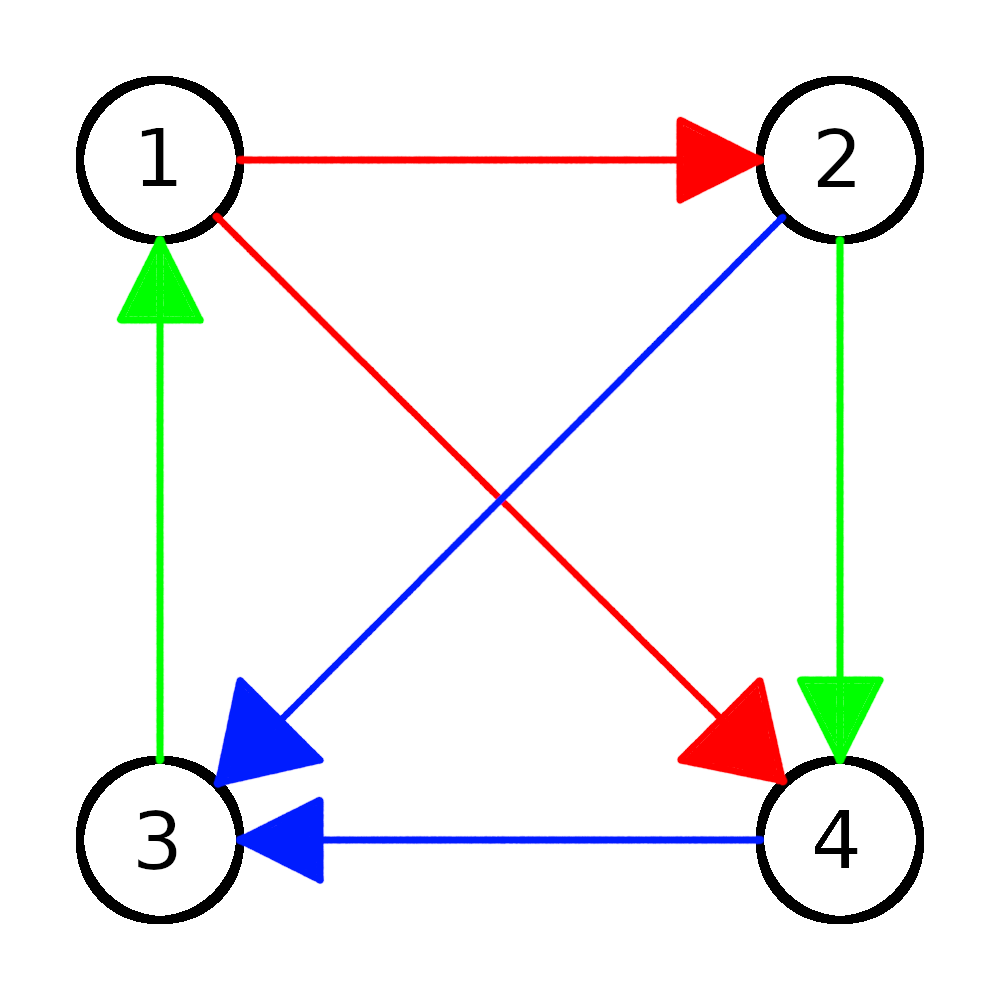
\includegraphics[scale=1]{pic/skcia3.png}
  
%%%%%%%%%%%%%%%%%%%%%%%%%%%%%%%%%%%%%%%%%%%%%%%%%%%%%%%%%%%%%%%%%%%%%%
% We're done
\end{statement}

%%% Local Variables:
%%% mode: latex
%%% mode: flyspell
%%% ispell-local-dictionary: "croatian"
%%% TeX-master: "../hio.tex"
%%% End: